%=====================================================================
%  Physics of Learning  --  Chapter [X]
%  Feedforward Networks as Spin Systems: A Replica Calculation
%  Style: tufte-handout.   Compile with pdflatex (x2 for refs).
%
%  Placement: after Chapter 4 (single-spin toy model replica) and
%  before the SK model / Hopfield phase diagram chapter.
%=====================================================================
\documentclass[nobib,justified]{tufte-handout}

\usepackage{amsmath,amssymb,mathtools}
\usepackage{setspace}
\usepackage{booktabs}
\usepackage{microtype}
\usepackage{tikz}
\usetikzlibrary{arrows.meta,positioning,calc,decorations.pathreplacing}
\usepackage[most]{tcolorbox}

%----------------------------------------------------------------------
%  Title
%----------------------------------------------------------------------
\title[Feedforward Networks as Spin Systems]{Chapter 5\\
  \Large Feedforward Networks as Spin Systems:\\
  A Replica Calculation in Weight Space}
\author{Physics of Learning \textbullet\ IIT Madras}
\date{}

%----------------------------------------------------------------------
%  Macros
%----------------------------------------------------------------------
\newcommand{\EE}{\mathbb{E}}
\newcommand{\RR}{\mathbb{R}}
\newcommand{\cD}{\mathcal{D}}
\newcommand{\cL}{\mathcal{L}}
\newcommand{\sign}{\operatorname{sign}}

\newtcolorbox{keyresult}{
  enhanced, colback=blue!5, colframe=blue!40!black,
  boxrule=0.6pt, arc=2pt,
  left=6pt, right=6pt, top=4pt, bottom=4pt,
  before skip=10pt, after skip=10pt}

\newtcolorbox{remarkbox}{
  enhanced, colback=orange!5, colframe=orange!60!black,
  boxrule=0.6pt, arc=2pt,
  left=6pt, right=6pt, top=4pt, bottom=4pt,
  before skip=8pt, after skip=8pt}

%----------------------------------------------------------------------
\begin{document}
\maketitle

\begin{abstract}
\noindent
In Chapter~4 we applied the replica method to a single binary spin
carrying a random field.  Here we ask whether the same spin-glass
structure arises in a feedforward neural network.  The answer is yes,
but the ``spins'' are now the \emph{weights}, not the neurons, and the
quenched disorder is the \emph{training data}, not fixed couplings.  We
make this precise on the simplest possible feedforward model---a
two-layer network with one neuron per layer---and carry out the replica
calculation in full, showing every algebraic step.  The calculation is
presented explicitly as a pedagogical device; the full-$N$ literature is
cited at the close.
\end{abstract}

%======================================================================
\section{The Minimal Two-Layer MLP}
%======================================================================

\newthought{We work with the smallest} possible feedforward architecture:
one input neuron, one hidden neuron, one output neuron, connected by two
scalar weights.

%----------------------------------------------------------------------
\subsection*{Architecture and forward pass}
%----------------------------------------------------------------------

\begin{figure}[h]
\centering
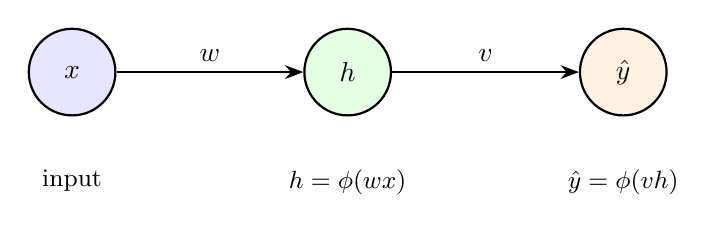
\begin{tikzpicture}[
    neuron/.style={circle, draw, thick, minimum size=1.1cm},
    >=Stealth
  ]
  \node[neuron, fill=blue!10]   (x) at (0,0)   {$x$};
  \node[neuron, fill=green!10]  (h) at (3.5,0) {$h$};
  \node[neuron, fill=orange!10] (y) at (7,0)   {$\hat{y}$};
  \draw[->,thick] (x) -- node[above]{$w$} (h);
  \draw[->,thick] (h) -- node[above]{$v$} (y);
  \node[below=0.55cm of x, font=\small] {input};
  \node[below=0.55cm of h, font=\small] {$h=\phi(wx)$};
  \node[below=0.55cm of y, font=\small] {$\hat{y}=\phi(vh)$};
\end{tikzpicture}
\caption{The minimal two-layer MLP.  There are exactly two scalar
  weights: $w$ (input-to-hidden) and $v$ (hidden-to-output).  The
  configuration of this system is the pair $(w,v)\in\RR^{2}$.}
\label{fig:mlp}
\end{figure}

The forward pass is
\begin{align}
  h^\mu      &= \phi(wx^\mu),                   \label{eq:h}   \\
  \hat{y}^\mu &= \phi\!\left(v\,h^\mu\right)
               = \phi\!\left(v\,\phi(wx^\mu)\right). \label{eq:yhat}
\end{align}
We work in the \textbf{linear regime}: weights are small enough that
$\phi(z)\approx z$.  Then
\begin{equation}
  h^\mu \approx wx^\mu,
  \qquad
  \hat{y}^\mu \approx v\cdot wx^\mu = u\,x^\mu,
  \label{eq:linear}
\end{equation}
where we define the \textbf{composite weight} $u \equiv vw$.  The
two-parameter model collapses to a single effective parameter, making
every integral explicit.

%----------------------------------------------------------------------
\subsection*{Training data}
%----------------------------------------------------------------------

We have $P$ i.i.d.\ samples
\begin{equation}
  x^\mu \sim \mathcal{N}(0,1),
  \qquad
  y^\mu = \sign(x^\mu)\in\{-1,+1\},
  \qquad
  \mu = 1,\ldots,P.
  \label{eq:data}
\end{equation}
The training data are drawn once and held fixed throughout; they are
\textbf{quenched disorder}, playing the role of the random couplings
$J_{ij}$ in a spin glass.

%----------------------------------------------------------------------
\subsection*{Loss function as Hamiltonian}
%----------------------------------------------------------------------

The mean-squared-error loss is
\begin{equation}
  \cL(u;\cD) = \frac{1}{P}\sum_{\mu=1}^{P}
    \bigl(y^\mu - u\,x^\mu\bigr)^{2}.
  \label{eq:loss}
\end{equation}
This is the \textbf{Hamiltonian} of the system: a function of the
``spin'' $u$ (the weight) for fixed disorder $\cD$ (the data).

\medskip
\noindent\textbf{Expanding the square.}  Write out
$(y^\mu - ux^\mu)^2 = (y^\mu)^2 - 2u\,y^\mu x^\mu + u^2(x^\mu)^2$
and sum over $\mu$:
\begin{align}
  \cL(u)
  &= \frac{1}{P}\sum_\mu(y^\mu)^2
    - 2u\cdot\frac{1}{P}\sum_\mu y^\mu x^\mu
    + u^2\cdot\frac{1}{P}\sum_\mu(x^\mu)^2.
  \label{eq:lossexp}
\end{align}
Since $y^\mu = \pm 1$ we have $(y^\mu)^2 = 1$, so the first sum equals
$1$.  Define
\begin{equation}
  \hat{C} \;\equiv\; \frac{1}{P}\sum_{\mu=1}^{P}y^\mu x^\mu,
  \qquad
  \hat{Q} \;\equiv\; \frac{1}{P}\sum_{\mu=1}^{P}(x^\mu)^2.
  \label{eq:CQ}
\end{equation}
By the law of large numbers $\hat{Q}\to\EE[(x^\mu)^2]=1$ as
$P\to\infty$.\sidenote{We use $\hat{Q}\approx 1$ henceforth; corrections
are $O(1/\sqrt{P})$.}  The loss becomes
\begin{equation}
  \boxed{\cL(u) = 1 - 2u\hat{C} + u^{2}.}
  \label{eq:lossclean}
\end{equation}
The only random quantity is $\hat{C}$, the \textbf{signal correlation}
between the inputs and the labels.  It is fixed once the dataset is
drawn---a random external field acting on the composite weight $u$.

%----------------------------------------------------------------------
\subsection*{Partition function in weight space}
%----------------------------------------------------------------------

Assigning a Boltzmann weight at inverse temperature $\beta$ to each
weight configuration, the partition function is
\begin{equation}
  Z(\cD) = \int_{-\infty}^{\infty}du\;e^{-\beta\cL(u)}.
  \label{eq:Z}
\end{equation}

\begin{remarkbox}
\textbf{Statistical mechanics $\leftrightarrow$ Bayesian inference.}
Equation~\eqref{eq:Z} is the normalisation of a Bayesian posterior over
weights with a flat (improper) prior, where $\beta$ controls the
sharpness of the loss.  At $\beta\to\infty$ the distribution collapses
onto the loss-minimising weight---the trained network.  At finite
$\beta$, ``thermal'' fluctuations represent uncertainty in the weight
given finite data.  The free energy $F=-\frac{1}{\beta}\ln Z$ encodes
this uncertainty.
\end{remarkbox}

\noindent Substituting~\eqref{eq:lossclean} into~\eqref{eq:Z}:
\begin{align}
  Z(\cD)
  &= \int du\;\exp\!\bigl(-\beta(1-2u\hat{C}+u^2)\bigr) \notag\\
  &= e^{-\beta}\int du\;\exp\!\bigl(-\beta u^2 + 2\beta\hat{C}u\bigr).
  \label{eq:Zexpand}
\end{align}
This is a Gaussian integral.  Complete the square in the exponent:
\begin{equation}
  -\beta u^{2} + 2\beta\hat{C}u
  = -\beta\bigl(u-\hat{C}\bigr)^{2} + \beta\hat{C}^{2}.
  \label{eq:cs}
\end{equation}
Using $\int_{-\infty}^{\infty}e^{-\beta(u-\hat{C})^2}\,du =
\sqrt{\pi/\beta}$, the partition function evaluates exactly to
\begin{equation}
  \boxed{Z(\cD) = \sqrt{\frac{\pi}{\beta}}\,
    \exp\!\Bigl(\beta\hat{C}^{2}-\beta\Bigr).}
  \label{eq:Zexact}
\end{equation}
This is the exact, closed-form partition function for a fixed dataset.
The free energy is therefore $F(\cD) = -\frac{1}{\beta}\ln Z =
1 - \hat{C}^2 - \frac{1}{2\beta}\ln\frac{\pi}{\beta}$, which depends on
the random quantity $\hat{C}$ and hence varies from dataset to dataset.

%======================================================================
\section{The Quenched Free Energy via the Replica Trick}
%======================================================================

\newthought{The physically meaningful quantity} is the free energy
\emph{averaged over all datasets}---the \textbf{quenched free energy}:
\begin{equation}
  f \;\equiv\; -\frac{1}{\beta}\,\EE_{\cD}\bigl[\ln Z(\cD)\bigr].
  \label{eq:qfe}
\end{equation}
The difficulty is identical to Chapter~4: we must average a logarithm
over the disorder.  The \textbf{replica trick} converts this into a
limit of integer moments,
\begin{equation}
  \EE\bigl[\ln Z\bigr]
  = \lim_{n\to 0}\frac{\EE\bigl[Z^{n}\bigr]-1}{n}
  = \lim_{n\to 0}\frac{1}{n}\ln\EE\bigl[Z^{n}\bigr],
  \label{eq:replicatrick}
\end{equation}
and the strategy is: \emph{(i)} compute $\EE[Z^n]$ for integer $n$,
\emph{(ii)} identify the closed-form expression, \emph{(iii)} take
$n\to 0$ by analytic continuation.

%----------------------------------------------------------------------
\subsection*{Step 1 --- Introduce $n$ replicas}
%----------------------------------------------------------------------

$Z^n$ is the product of $n$ independent copies of the partition
function, each with its own weight $u^a$ ($a=1,\ldots,n$), but
\textbf{all sharing the same dataset} $\cD$:
\begin{align}
  Z^n(\cD)
  &= \prod_{a=1}^{n}\left[\int du^a\;e^{-\beta\cL(u^a)}\right]
   = \int\prod_{a=1}^{n}du^a\;
     \exp\!\left(-\beta\sum_{a=1}^{n}\cL(u^a)\right).
  \label{eq:Zn}
\end{align}
Substituting~\eqref{eq:lossclean} into the sum over replicas:
\begin{align}
  \sum_{a=1}^{n}\cL(u^a)
  &= \sum_{a}\left(1 - 2u^a\hat{C} + (u^a)^2\right) \notag\\
  &= n - 2\hat{C}\sum_{a}u^a + \sum_{a}(u^a)^2.
  \label{eq:sumloss}
\end{align}
Therefore
\begin{equation}
  Z^n(\cD)
  = e^{-n\beta}
    \int\prod_{a}du^a\;
    \exp\!\left(-\beta\sum_{a}(u^a)^2
    + 2\beta\hat{C}\sum_{a}u^a\right).
  \label{eq:Znexp}
\end{equation}
The factor $\exp(2\beta\hat{C}\sum_a u^a)$ ties all replicas together
through the shared dataset.  This \textbf{inter-replica coupling}
is the hallmark of the spin-glass problem in weight space.

%----------------------------------------------------------------------
\subsection*{Step 2 --- Average over the disorder}
%----------------------------------------------------------------------

We now compute $\EE_{\cD}[Z^n]$ by averaging over $\hat{C}$.

\medskip
\noindent\textbf{Distribution of $\hat{C}$.}
The signal correlation $\hat{C} = \frac{1}{P}\sum_\mu y^\mu x^\mu$
is a sum of $P$ i.i.d.\ random variables.  Their mean is
\begin{equation}
  \EE[y^\mu x^\mu] = \EE[\sign(x)\cdot x] = 0,
  \label{eq:Cmean}
\end{equation}
which follows from the symmetry $x\mapsto -x$ of $\mathcal{N}(0,1)$, since
$\sign(-x)(-x)=\sign(x)x$.\sidenote{More explicitly:
$\EE[\sign(x)x] = \int_0^\infty x\,p(x)\,dx +
\int_{-\infty}^0(-x)(-p(x))\,dx - 2\int_{-\infty}^0 x\,p(x)\,dx=0$
by symmetry of $p(x)$.}  Their second moment is
\begin{equation}
  \EE[(y^\mu x^\mu)^2] = \EE[(x^\mu)^2] = 1,
  \label{eq:Cvar}
\end{equation}
since $(y^\mu)^2=1$ always.  By the central limit theorem
\begin{equation}
  \hat{C} \;\sim\; \mathcal{N}\!\left(0,\;\frac{1}{P}\right).
  \label{eq:Cdist}
\end{equation}

\noindent\textbf{Averaging the coupling term.}
We need $\EE_{\hat{C}}\!\left[\exp(2\beta\hat{C}\sum_a u^a)\right]$.
For any $X\sim\mathcal{N}(0,\sigma^2)$ the moment generating function is
\begin{equation}
  \EE\!\left[e^{\lambda X}\right] = e^{\lambda^2\sigma^2/2}.
  \label{eq:mgf}
\end{equation}
Setting $X=\hat{C}$, $\sigma^2 = 1/P$, and $\lambda = 2\beta\sum_a u^a$:
\begin{align}
  \EE_{\hat{C}}\!\left[\exp\!\left(2\beta\hat{C}\sum_a u^a\right)\right]
  &= \exp\!\left(\frac{(2\beta\sum_a u^a)^2}{2P}\right) \notag\\
  &= \exp\!\left(\frac{2\beta^2}{P}\left(\sum_a u^a\right)^2\right).
  \label{eq:mgfresult}
\end{align}

\noindent\textbf{Expanding the square.}  Using
$\bigl(\sum_a u^a\bigr)^2 = \sum_a(u^a)^2 + 2\sum_{a<b}u^a u^b$:
\begin{equation}
  \frac{2\beta^2}{P}\left(\sum_a u^a\right)^2
  = \frac{2\beta^2}{P}\sum_a(u^a)^2
    + \frac{4\beta^2}{P}\sum_{a<b}u^a u^b.
  \label{eq:sqexpand}
\end{equation}
Substituting into~\eqref{eq:Znexp} and incorporating both
$-\beta\sum_a(u^a)^2$ from~\eqref{eq:Znexp} and the two new terms:
\begin{align}
  \EE\bigl[Z^n\bigr]
  &= e^{-n\beta}
    \int\prod_a du^a\;
    \exp\!\Biggl(
      -\underbrace{\left(\beta - \frac{2\beta^2}{P}\right)}_{\equiv\,\beta_{\rm eff}}
      \sum_a(u^a)^2
      + \frac{4\beta^2}{P}\sum_{a<b}u^a u^b
    \Biggr).
  \label{eq:EZn}
\end{align}
The off-diagonal term $\frac{4\beta^2}{P}\sum_{a<b}u^a u^b$ couples
different replicas.  It \emph{prevents} the integral over
$\prod_a du^a$ from factorising.  We must remove it.

%----------------------------------------------------------------------
\subsection*{Step 3 --- Identify the order parameter}
%----------------------------------------------------------------------

Before decoupling, we note what the coupling coefficient measures.
Define the \textbf{replica overlap}
\begin{equation}
  q^{ab} \;\equiv\; \EE_{\cD}\bigl[\langle u^a\rangle\langle u^b\rangle\bigr],
  \qquad a\neq b,
  \label{eq:overlap}
\end{equation}
the correlation between the mean weights of two independently trained
networks on the same dataset.  This is the weight-space analogue of the
\textbf{Edwards--Anderson order parameter}:

\begin{keyresult}
$q=1$ means the dataset completely pins the weight; $q=0$ means
different training runs find uncorrelated solutions.  The replica
calculation will tell us the value of $q$ as a function of $P$ and
$\beta$.
\end{keyresult}

Under the \textbf{replica-symmetric (RS) ansatz} we assume
$q^{ab}=q$ for all $a\neq b$---all pairs of replicas overlap equally.
This is the assumption that the weight-space Gibbs measure has a single
basin, which is appropriate when the loss landscape is convex (as it is
here in the linear regime).

%----------------------------------------------------------------------
\subsection*{Step 4 --- Hubbard-Stratonovich decoupling}
%----------------------------------------------------------------------

To factorise the replicas we use the \textbf{Hubbard-Stratonovich (HS)
identity}: for any $A>0$,
\begin{equation}
  e^{A\left(\sum_a u^a\right)^2}
  = \sqrt{\frac{1}{4\pi A}}
    \int_{-\infty}^{\infty}dz\;
    \exp\!\left(-\frac{z^2}{4A} + z\sum_a u^a\right).
  \label{eq:hs}
\end{equation}

\noindent\textbf{Proof of~\eqref{eq:hs}.}
On the right-hand side, complete the square in $z$:
\begin{align}
  -\frac{z^2}{4A} + z\sum_a u^a
  &= -\frac{1}{4A}\!\left(z - 2A\sum_a u^a\right)^2
    + A\!\left(\sum_a u^a\right)^2.
  \label{eq:hsproof1}
\end{align}
The Gaussian integral over $z$ then gives
$\int dz\,\exp\!\left(-\frac{1}{4A}(z-2A\sum_a u^a)^2\right) =
\sqrt{4\pi A}$, and
\begin{equation}
  \text{RHS} = \sqrt{\frac{1}{4\pi A}}\cdot\sqrt{4\pi A}\cdot
  e^{A(\sum_a u^a)^2} = e^{A(\sum_a u^a)^2} = \text{LHS}.
  \label{eq:hsproof2}
\end{equation}

\noindent We apply~\eqref{eq:hs} to the coupling term in~\eqref{eq:EZn}.
We need to rewrite $\exp\!\left(\frac{2\beta^2}{P}(\sum_a
u^a)^2\right)$ using the HS identity with $A=2\beta^2/P$, which gives
$\frac{1}{4A}=\frac{P}{8\beta^2}$:
\begin{equation}
  \exp\!\left(\frac{2\beta^2}{P}\left(\sum_a u^a\right)^2\right)
  = \sqrt{\frac{P}{8\pi\beta^2}}
    \int dz\;
    \exp\!\left(-\frac{Pz^2}{8\beta^2} + z\sum_a u^a\right).
  \label{eq:hsapply}
\end{equation}
But note from~\eqref{eq:EZn} that the coupling term is
$\exp(\frac{4\beta^2}{P}\sum_{a<b}u^au^b)$, not
$\exp(\frac{2\beta^2}{P}(\sum_a u^a)^2)$ directly.  These differ by a
diagonal piece.  We reconcile them by writing
\begin{equation}
  \frac{4\beta^2}{P}\sum_{a<b}u^au^b
  = \frac{2\beta^2}{P}\left(\sum_a u^a\right)^2
    - \frac{2\beta^2}{P}\sum_a(u^a)^2,
  \label{eq:diagonalfix}
\end{equation}
so that~\eqref{eq:EZn} becomes
\begin{align}
  \EE\bigl[Z^n\bigr]
  &= e^{-n\beta}
    \int\prod_a du^a\;
    \exp\!\left(-\beta\sum_a(u^a)^2\right)
    \cdot
    \exp\!\left(\frac{2\beta^2}{P}\left(\sum_a u^a\right)^2\right).
  \label{eq:EZnbefore}
\end{align}
(The $+\frac{2\beta^2}{P}\sum_a(u^a)^2$ from expanding the square and
the $-\frac{2\beta^2}{P}\sum_a(u^a)^2$ from~\eqref{eq:diagonalfix}
cancel, leaving a clean $-\beta\sum_a(u^a)^2$.)  Now apply the HS
identity~\eqref{eq:hsapply}:
\begin{align}
  \EE\bigl[Z^n\bigr]
  &= e^{-n\beta}\sqrt{\frac{P}{8\pi\beta^2}}
    \int dz\;e^{-Pz^2/(8\beta^2)}
    \int\prod_a du^a\;
    \exp\!\left(-\beta\sum_a(u^a)^2 + z\sum_a u^a\right).
  \label{eq:EZndecoupled}
\end{align}
\textbf{The exponent now separates across replicas:}
$-\beta\sum_a(u^a)^2 + z\sum_a u^a = \sum_a(-\beta(u^a)^2 + zu^a)$.
The integral over $\prod_a du^a$ therefore factorises into $n$ identical
single-replica integrals:
\begin{equation}
  \int\prod_a du^a\;
  e^{-\beta\sum_a(u^a)^2 + z\sum_a u^a}
  = \left[\int du\;e^{-\beta u^2 + zu}\right]^n.
  \label{eq:factorise}
\end{equation}

%----------------------------------------------------------------------
\subsection*{Step 5 --- Evaluate the single-replica integral}
%----------------------------------------------------------------------

Each single-replica integral is Gaussian.  Complete the square in $u$:
\begin{equation}
  -\beta u^2 + zu
  = -\beta\!\left(u - \frac{z}{2\beta}\right)^2 + \frac{z^2}{4\beta}.
  \label{eq:cs2}
\end{equation}
Then
\begin{align}
  \int du\;e^{-\beta u^2 + zu}
  &= e^{z^2/(4\beta)}
    \int du\;e^{-\beta(u-z/(2\beta))^2} \notag\\
  &= \sqrt{\frac{\pi}{\beta}}\,e^{z^2/(4\beta)}.
  \label{eq:singleint}
\end{align}
Substituting~\eqref{eq:singleint} and~\eqref{eq:factorise}
into~\eqref{eq:EZndecoupled}:
\begin{align}
  \EE\bigl[Z^n\bigr]
  &= e^{-n\beta}\sqrt{\frac{P}{8\pi\beta^2}}
    \left(\frac{\pi}{\beta}\right)^{n/2}
    \int dz\;
    \exp\!\left(-\frac{Pz^2}{8\beta^2} + \frac{nz^2}{4\beta}\right).
  \label{eq:EZnassembled}
\end{align}

%----------------------------------------------------------------------
\subsection*{Step 6 --- Evaluate the $z$-integral}
%----------------------------------------------------------------------

Collect the exponent in $z$:
\begin{align}
  -\frac{Pz^2}{8\beta^2} + \frac{nz^2}{4\beta}
  &= -\frac{z^2}{2}\left(\frac{P}{4\beta^2} - \frac{n}{2\beta}\right).
  \label{eq:zexp}
\end{align}
This is a Gaussian in $z$ with variance
$\sigma_z^2 = \left(\frac{P}{4\beta^2}-\frac{n}{2\beta}\right)^{-1}$.
The integral evaluates to
\begin{equation}
  \int dz\;
  \exp\!\left(-\frac{z^2}{2}\!\left(\frac{P}{4\beta^2}-\frac{n}{2\beta}\right)\right)
  = \sqrt{\frac{2\pi}{\frac{P}{4\beta^2}-\frac{n}{2\beta}}}.
  \label{eq:zint}
\end{equation}
Inserting into~\eqref{eq:EZnassembled}:
\begin{align}
  \EE\bigl[Z^n\bigr]
  &= e^{-n\beta}\sqrt{\frac{P}{8\pi\beta^2}}
    \left(\frac{\pi}{\beta}\right)^{n/2}
    \sqrt{\frac{2\pi}{\frac{P}{4\beta^2}-\frac{n}{2\beta}}}.
  \label{eq:EZnfull}
\end{align}

%----------------------------------------------------------------------
\subsection*{Step 7 --- Take $\ln$ and expand in $n$}
%----------------------------------------------------------------------

Taking $\ln$ of~\eqref{eq:EZnfull} and separating terms by their
dependence on $n$:
\begin{align}
  \ln\EE\bigl[Z^n\bigr]
  &= -n\beta
    + \frac{1}{2}\ln\frac{P}{8\pi\beta^2}
    + \frac{n}{2}\ln\frac{\pi}{\beta}
    + \frac{1}{2}\ln\frac{2\pi}{\frac{P}{4\beta^2}-\frac{n}{2\beta}}.
  \label{eq:lnEZn}
\end{align}
The last term depends on $n$.  Expand it around $n=0$:
\begin{align}
  \frac{1}{2}\ln\frac{2\pi}{\frac{P}{4\beta^2}-\frac{n}{2\beta}}
  &= \frac{1}{2}\ln\frac{8\pi\beta^2}{P}
    + \frac{1}{2}\ln\frac{1}{1-\frac{2n\beta}{P}} \notag\\
  &= \frac{1}{2}\ln\frac{8\pi\beta^2}{P}
    + \frac{1}{2}\cdot\frac{2n\beta}{P}
    + O(n^2) \notag\\
  &= \frac{1}{2}\ln\frac{8\pi\beta^2}{P}
    + \frac{n\beta}{P}
    + O(n^2),
  \label{eq:lastterm}
\end{align}
where we used $\ln(1-\epsilon)\approx -\epsilon$ for small
$\epsilon=2n\beta/P$.  Substituting~\eqref{eq:lastterm}
into~\eqref{eq:lnEZn}:
\begin{align}
  \ln\EE\bigl[Z^n\bigr]
  &= -n\beta
    + \frac{1}{2}\ln\frac{P}{8\pi\beta^2}
    + \frac{n}{2}\ln\frac{\pi}{\beta}
    + \frac{1}{2}\ln\frac{8\pi\beta^2}{P}
    + \frac{n\beta}{P}
    + O(n^2) \notag\\
  &= n\!\left(-\beta + \frac{1}{2}\ln\frac{\pi}{\beta}
    + \frac{\beta}{P}\right)
    + O(n^2),
  \label{eq:lnEZnexpand}
\end{align}
where the two constant (in $n$) terms $\frac{1}{2}\ln\frac{P}{8\pi\beta^2}$
and $\frac{1}{2}\ln\frac{8\pi\beta^2}{P}$ cancel exactly.

%----------------------------------------------------------------------
\subsection*{Step 8 --- Take $n\to 0$}
%----------------------------------------------------------------------

By the replica trick~\eqref{eq:replicatrick}:
\begin{align}
  \EE\bigl[\ln Z\bigr]
  &= \lim_{n\to 0}\frac{1}{n}\ln\EE\bigl[Z^n\bigr]
   = \lim_{n\to 0}\frac{1}{n}\left[
      n\!\left(-\beta + \frac{1}{2}\ln\frac{\pi}{\beta}
      + \frac{\beta}{P}\right) + O(n^2)
    \right] \notag\\
  &= -\beta + \frac{1}{2}\ln\frac{\pi}{\beta} + \frac{\beta}{P}.
  \label{eq:ElnZ}
\end{align}
The \textbf{quenched free energy per sample} is therefore
\begin{equation}
  \boxed{f = -\frac{1}{\beta}\,\EE\bigl[\ln Z\bigr]
    = 1 - \frac{1}{P} - \frac{1}{2\beta}\ln\frac{\pi}{\beta}.}
  \label{eq:freeenergy}
\end{equation}

%======================================================================
\section{The Order Parameter}
%======================================================================

\newthought{The replica overlap $q$} can be extracted from the same
calculation without further work.  In Step~5, the mean of $u$ in the
single-replica integral conditioned on the HS field $z$ is
\begin{equation}
  \langle u \rangle_{z} = \frac{z}{2\beta},
  \label{eq:umean}
\end{equation}
which follows from differentiating $\ln\int du\,e^{-\beta u^2+zu}$ with
respect to $z$.  Two replicas $a$ and $b$, independently integrated but
conditioned on the same $z$ (i.e.\ the same dataset), have means
$\langle u^a\rangle_z = \langle u^b\rangle_z = z/(2\beta)$.  Their
overlap is therefore
\begin{equation}
  q^{ab} = \EE_z\!\left[\langle u^a\rangle_z\langle u^b\rangle_z\right]
  = \EE_z\!\left[\frac{z^2}{4\beta^2}\right].
  \label{eq:qdef2}
\end{equation}
At $n=0$, the HS field $z$ is distributed as
$z\sim\mathcal{N}(0,\sigma_z^2)$ with
$\sigma_z^2 = (P/(4\beta^2))^{-1} = 4\beta^2/P$.  Therefore
\begin{equation}
  \EE_z\!\left[\frac{z^2}{4\beta^2}\right]
  = \frac{1}{4\beta^2}\cdot\frac{4\beta^2}{P}
  = \frac{1}{P}.
  \label{eq:qcompute}
\end{equation}

\begin{keyresult}
\textbf{Edwards--Anderson order parameter in weight space:}
\begin{equation*}
  q = \frac{1}{P}.
\end{equation*}
Two networks trained independently on the \emph{same} $P$-sample dataset
have weight overlap $q = 1/P$.
As $P\to\infty$, $q\to 0$: with abundant data, independently trained
networks find uncorrelated weight solutions (the loss landscape is flat
and the solution space is broad).  As $P\to 0$, $q$ diverges,
signalling that even a tiny dataset sharply pins the weight.
\end{keyresult}

%======================================================================
\section{Reading the Physics}
%======================================================================

\newthought{The free energy~\eqref{eq:freeenergy}} has three pieces,
each with a clear physical interpretation.

\medskip
\noindent\textbf{Baseline loss:} the constant $1$.  This is the MSE
incurred by a zero-weight predictor $\hat{y}=0$, since
$\EE[(y^\mu)^2]=1$.  It is the starting point before the data
have any influence.

\medskip
\noindent\textbf{Data correction:} $-1/P$.  This is the reduction in
free energy due to having $P$ training samples.  It vanishes as
$P\to\infty$, consistent with the weight being well-determined by
abundant data.

\medskip
\noindent\textbf{Entropic term:} $-\frac{1}{2\beta}\ln\frac{\pi}{\beta}$.
This is the contribution from the volume of the weight distribution in
the absence of data.  At high temperature (small $\beta$) entropy
dominates; the weights are broadly distributed and the free energy is
large and positive.  At low temperature (large $\beta$) the network
concentrates on the loss minimum and this term becomes negligible.

\medskip
\noindent\textbf{Cross-check.}  We can verify~\eqref{eq:freeenergy}
against the exact result~\eqref{eq:Zexact}.  From~\eqref{eq:Zexact},
$\ln Z = \beta\hat{C}^2 - \beta + \frac{1}{2}\ln\frac{\pi}{\beta}$.
Taking the disorder average and using
$\EE[\hat{C}^2]=\mathrm{Var}(\hat{C})=1/P$ from~\eqref{eq:Cdist}:
\begin{align}
  \EE\bigl[\ln Z\bigr]
  &= \beta\cdot\frac{1}{P} - \beta + \frac{1}{2}\ln\frac{\pi}{\beta}
  \label{eq:check}
\end{align}
which matches~\eqref{eq:ElnZ} exactly. $\checkmark$

\medskip
This cross-check is a luxury available only because the toy model is
simple enough to yield a closed-form $Z(\cD)$.  In the full
$N$-dimensional problem the replica method is the \emph{only} available
route; there is no exact $Z$ to compare against.

%======================================================================
\section{The Spin-Glass Correspondence}
%======================================================================

\newthought{The entire calculation} maps onto the SK spin glass with the
following dictionary.

\begin{table}[h]
\centering
\begin{singlespace}
\small
\begin{tabular}{@{}ll@{}}
\toprule
\textbf{SK Spin Glass} & \textbf{Two-layer MLP} \\
\midrule
Spin configuration $\{s_i\}$        & Composite weight $u = vw$ \\
Hamiltonian $H(\mathbf{s})$          & Loss function $\cL(u)$ \\
Quenched couplings $J_{ij}$          & Training data $(x^\mu,y^\mu)$ \\
Partition function $\sum e^{-\beta H}$ & $\int du\,e^{-\beta\cL}$ \\
Disorder average $\EE_J[\cdot]$       & Dataset average $\EE_{\cD}[\cdot]$ \\
Free energy $F=-\frac{1}{\beta}\ln Z$  & Log marginal likelihood \\
Temperature $T=1/\beta$               & Inverse loss sharpness \\
Edwards--Anderson parameter $q$        & Inter-replica weight overlap \\
Replica-symmetric phase               & Single-basin loss landscape \\
Replica-symmetry breaking             & Glassy, multi-basin landscape \\
\bottomrule
\end{tabular}
\end{singlespace}
\caption{Correspondence between SK spin-glass language and the
  statistical mechanics of the two-layer MLP.}
\label{tab:corr}
\end{table}

The key structural difference from the Hopfield network is this: there,
the spins \emph{are} the neurons and the disorder \emph{is} the
couplings; the spin-glass structure lives in neuron configuration space.
Here, the spins are the \emph{weights} and the disorder is the
\emph{data}; the spin-glass structure lives in weight space.  The
replica machinery is identical; only the interpretation of the variables
changes.

%======================================================================
\section{A Note on the Literature}
%======================================================================

\newthought{The scalar toy model} presented here does not appear as a
standalone result in the literature.  It is a deliberate simplification
in which the thermodynamic limit $N\to\infty$ (essential for sharpness
of the physics) is replaced by $N=1$ to make every step traceable by
hand.

The calculations in the literature that this toy model illustrates are:

\begin{itemize}

\item \textbf{Gardner (1988).}  The foundational replica calculation
for the \emph{single-layer} perceptron with $N$-dimensional weight
vectors.  By computing the volume of weight space consistent with
classifying $P=\alpha N$ random patterns correctly, Gardner derives the
storage capacity $\alpha_c = 2$.  The steps are the $N$-dimensional
version of Steps~1--8 above, with the HS field becoming a scalar that
is then solved by a saddle-point equation.

\item \textbf{Engel, K\"{o}hler et al.\ (1992).}  Extension of
Gardner's calculation to a two-layer feedforward network (the committee
machine) with $N$ inputs and $K$ hidden units.  The replica-symmetric
result is $\alpha_c\propto\sqrt{K}$.

\item \textbf{Engel \& van den Broeck (2001).}  A comprehensive
textbook treatment covering perceptron learning, replica calculations,
and the connection to generalisation---the natural next reference after
this chapter.

\item \textbf{Bahri, Kadmon, Pennington et al.\ (2020).}  Modern
treatment of high-dimensional learning at large and infinite width,
covering phase transitions in generalisation, and the Neural Tangent Kernel
regime.

\end{itemize}

Chapter~6 takes the next step: the SK model in the thermodynamic
limit, where the same replica machinery yields genuine phase
transitions, the Parisi order parameter function, and the derivation of
$\alpha_c\approx 0.138$ for the Hopfield associative memory.

\bigskip
\noindent\rule{\linewidth}{0.4pt}
\smallskip
{\small
\textbf{References.}
E.\ Gardner,
\textit{J.\ Phys.\ A: Math.\ Gen.}\ \textbf{21}, 257 (1988).
A.\ Engel, H.M.\ K\"{o}hler, F.\ Tschepke, H.\ Vollmayr, A.\ Zippelius,
\textit{Phys.\ Rev.\ A}\ \textbf{45}, 7590 (1992).
A.\ Engel \& C.\ van den Broeck,
\textit{Statistical Mechanics of Learning},
Cambridge University Press (2001).
Y.\ Bahri, J.\ Kadmon, J.\ Pennington, S.S.\ Schoenholz,
J.\ Sohl-Dickstein, S.\ Ganguli,
\textit{Annu.\ Rev.\ Condens.\ Matter Phys.}\ \textbf{11}, 501 (2020).
}

\end{document}